% \documentclass{report}
% \usepackage[utf8]{inputenc}
% \usepackage{booktabs}
% \usepackage[top=1.12in, bottom=1.62in, left=1.7in, right=1.7in]{geometry}
% \usepackage{graphicx}
% \usepackage[section]{placeins}

% \title{Final}
% \author{markkasun }
% \date{April 2016}

% \begin{document}

\chapter{Introduction}
Weighted Set Cover is a very popular NP-Hard problem which has a few different forms that include just set cover, where all weights are set to one and other forms such as vertex cover. There are many important algorithmic problems that can be formulated as set cover and that’s why an approximation algorithm found will be used for many problems (Kleinberg, 2005). There have been many attempts at finding a feasible solution to the problem but it remains unsolved. It has proven to be NP-Complete in decision form; Richard Manning Karp showed in his 1972 paper “Reducibility Among Combinatorial Problems” that there is a polynomial time reduction from SAT to Set Cover, and thus it is NP-Complete. Solving the Weighted Set Cover in P time means that P = NP. In the pursuit of such solutions, approximation algorithms and heuristics have been developed. Theses approximation algorithms and heuristics are used in real life applications of problems that can be transformed to weighted set cover. Real world applications of weighted set cover include choosing the smallest possible set of short sentences to tune all the features in a speech recognition software. In our presentation, we talked about how IBM found that searching only so many subsets of strings would lead them to finding all the viruses instead of searching the large number of viruses. Numerous other examples include finding a good location for facilities to set up, different scheduling problems, and resource allocation. The study of weighted set cover led to the development of fundamental techniques for the entire field of approximation algorithms (Kleinberg, 2005). Our report will discuss three algorithms for solving the Set Cover problem: greedy approximation, greedy heuristic, and simulated annealing.

The greedy approximation algorithm is efficient and provides a guaranteed cost when compared with the optimal solution. The greedy heuristic is extremely efficient and is used as the basis for the Simulated Annealing algorithm. Simulated Annealing is based on a method called annealing where in physical systems one guides a material to a crystalline state by gradually cooling an object from a high temperature state giving it time time to reach an equilibrium (Kleinberg 2005). Simulated annealing generates a random solution with a cost c(s) and then generates a solution from the neighbour and if that cost is less we take that solution and if not we may take the solution. We only take the solution of the cost if its higher depending on a certain probability.

For the experimental results, our group is using the OR-Library as our source of test data to run our algorithms against. The library contains and extensive list of different types of sets, that when tested on different algorithms will work better or worse. The library contains many different instances of weighted set cover problems. We will use the results of these tests to compare the effectiveness of the algorithms in terms of solutions given and time to arrive at those solutions. We will now define formally weighted set cover and show three methods for solving an instance of set cover.

\chapter{Problem Definition}
We first define the problem of set cover as Given a Set $E = \{e_1, e_2, \ldots ,e_n\}$ of $n$ elements, a collection of $m$ subsets $S_1, S_2, \ldots ,S_m$ of $E$ with weights $w_1, w_2, \ldots, w_m$. The goal to find a set $I \subset \{S_i, \ldots, S_m\}$ such that all elements covered by $I$ and the sum of the weights in $I$ is minimized. In decision form the problem is defined as: can we find a set cover with weight at most $W$. The optimal solution is two subsets, the two subsets chosen are the two horizontal subsets.\\
Example:\\
Assume weight of each subset is 1\\
Find the minimal set cover.\\
In decision form it is: Does there exist a set cover of weight W?

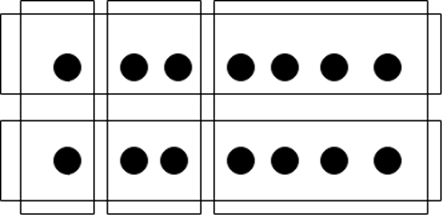
\includegraphics[width=.5\textwidth]{SetCoverExample}

\section{Greedy Approximation Algorithm}
The greedy approximation algorithm provides a guarantee when compared with the optimal solution to the problem. Unlike most approximation algorithms, the guarantee is not a constant multiple of the optimal but instead a it is a function multiple of the optimal based on the size of the input for the instance. The greedy approximation algorithm is guaranteed provide a solution that is less than or equal to $\alpha \cdot OPT(I)$ where $\alpha$ is given by $$\alpha = H_k = \sum_{i=1}^k \frac{1}{i}\leq 1+\log(k)$$ where $k$ is the size of the largest subset and $H_k$ is the $k$th partial sum of the harmonic series. Since $k$ will always be less than $n$, we can re-frame $\alpha$ in terms of $n$ if so desired. The proof of this is given by David S. Johnson but is too complicated for the scope of this report %\footnote{Johnson, p. 265-269}(Johnson, 1974, p. 265-269).

The guarantee of $H_k\cdot OPT(I)$ seems weak compared to algorithms for other NP-Hard problems where there are 2-approximation guarantees and even 3/2-approximations. The harmonic series quickly increases past 2 (passing it at $k=4$) and surpasses a guarantee of $3\times OPT$ at $k=11$. However, it has been shown that the efficiency of the greedy algorithm for general set cover problems cannot be improved to a constant nor to anything significantly more efficient than the greedy algorithm %\footnote{Pusztai, p. 408-409} (Pusztai, 2008, p. 408-409). The effectiveness of this guarantee in practice will be examined in the experimental results section where we will calculate guarantee for numerous test sets and compare with the actual result given by the greedy approximation algorithm.

The implementation of this algorithm is fairly simple and is given below in pseudo code. The actual implementation can be examined in the included code or github source repository (the greedy\textunderscore set\textunderscore cover function in main.py within the GreedySetCover directory). In the pseudo code, C represents the set of covered elements, X represents the list of chosen subsets.\\
Initialize $C=\{\}$, $X=[]$\\
While $|C| \neq |U|$\\
Find sub-set $S$ with smallest cost effectiveness (cost of $S$ divided by uncovered elements)\\
Set $C=C \cup S$\\
Add $S$ to $X$\\
Output X

Referring to the example given previously, there are 14 elements and 5 subsets where the weights of each subset is one. The optimal solution is to choose the two horizontal subsets while the greedy approximation algorithm will choose the three vertical subsets as they will consistently have better cost effectiveness at each iteration. The guarantee of the greedy approximation algorithm on this problem is $5.4\times OPT$ which is more than the total number of subsets in the problem. This example does not give much hope for the reliability of the guarantee for the approximation algorithm.

The greedy approximation algorithm also works on unweighted set cover where the weights of each subset is simply 1. The algorithm has a worst-case running time of $O(N\log(N))$ where $N$ is the actual size of the input including all subsets.

\section{Greedy Heuristic}\label{sec:heur}

Our heuristic algorithm is intended to quickly find an initial feasible solution and to construct neighbouring solutions for Simulated Annealing in a randomized manner. To this end we employ a fast greedy method proposed by Balas and Ho in 1987\todo{cite}.

This algorithm is intended for weighted set covering problems in particular, and aims to exploit the array of set costs -- and little else. It first greedily seeks the cheapest sets which help it to complete the cover by randomly choosing uncovered elements and selecting precisely the cheapest set which covers it. Usually, a combination of sets chosen later will include earlier sets as a subset, so that the latter become redundant. In order to capitalize on redundancies the algorithm greedily seeks expensive sets which can be removed without making the cover infeasible. It does this by iterating over the sets which were added to construct the cover in reverse order of their addition, and removes them if possible. This is summarized in the pseudocode below.
\begin{itemize}
    \item Initialize $C=\{\}$ and $X=[]$
    \item While $|C| \neq |U|$
    \begin{itemize}
        \item Pick a random element in $C$, and find the set $S$ of minimal cost which covers the element
        \item Let $C = C \cup S$ and append $S$ to $X$
    \end{itemize}
    \item Examine each selected set, in order by recency of selection. If the set is redundant -- that is, it can be removed without leaving an element uncovered -- remove it.
    \item Return the cover $X$.
\end{itemize}

The order of addition of sets is important to this algorithm. Cheap sets which cover many elements are statistically more likely to be added earlier, since there are more elements whose random selection prescribes the selection of these sets. Thus the algorithm discerns some statistical information about the cost effectiveness of the sets without performing any calculation, which is expressed in the order of the sets and exploited in the reduction by iterating in reverse. In essence, since the later sets added to build a complete cover are less likely to have a high cost-effectiveness, we are more likely to reduce to a cost-effective cover if we judge the later sets first.

While this algorithm has no performance guarantee, it scales better than the approximation algorithm since it does not compute cost-effectiveness across sets at each addition; yet it still exploits cost effectiveness in an implicit statistical manner, and performs better than the ``take the cheapest'' greedy idea would lead one to expect.

Our implementation of this algorithm has been written with its application as a subroutine of Simulated Annealing firmly in mind. As such, we have presumed a preprocessing step precedes the algorithm which sorts the array of costs in nondecreasing order, and indexes the sets accordingly; this is referred to in literature, \eg as by~\cite{JacobsBrusco}, as the ``natural order'' of the weighted set covering problem specification, and is the format used by our test problems from the OR Library. In fact, the OR library format can be described as a column-wise list-of-lists sparse representation of the problem's unweighted hypergraph adjacency matrix in a natural-order basis, such that we know the set of sets which cover each element in order of their cost. These problems are then already in the optimal format for application of the heuristic algorithm, and our implementation benefits from this -- while the approximation algorithm does not.

\section{Simulated Annealing}

NP-Hard optimization problems with NP-Complete decision problem analogs are characterized by an objective function which is easy to evaluate at a point but a ``search space'' of feasible solutions which is exponentially large in the size of the problem. Local search is a strategy which attempts to find a good solution quickly by iteratively evaluating feasible solutions which are in some heuristic sense similar to the present solution -- in its ``neighbourhood'' -- and choosing solutions which are an improvement on the present. An ideal local search algorithm thereby works toward optimality while evaluating only an exponentially smaller subset of the search space---but inevitably will converge to a a point which is only optimal with respect to its immediate neighbours. Our Heuristic and Approximation algorithms apply different local search strategies to the minimum weighted set covering problem, and in our tests find results fairly close to the global minimum, but very rarely attain it.

Metaheuristics are algorithms which augment local search with global information, progressively divining the structure of the search space from local search results and guiding the local searches towards the optimal. In order to improve on the performance of our algorithms, we guide the local search with an annealing metaheuristic; that is, one which allows selection of inferior neighbouring solutions prescribed according to a ``computational temperature'' parameter whose magnitude corresponds to a ``smoothing'' of the neighbourhood structure which the local search algorithm imposes on the search space. Of the varieties of annealing metaheuristics, we choose Simulated Annealing (SA) due~\cite{Kirkpatrick671}, which was the first annealing method used in optimization and has remained the most popular. The SA pseudocode follows:
\begin{itemize}
    \item GENERATE an initial solution $X$
    \item for $T$ in schedule:
    \begin{itemize}
        \item SEARCH for a neighbour solution $X'$
        \item let $\Delta = cost(X) - cost(X')$
        \item if $\Delta < 0$ or rand(0, 1] < $\exp(-\frac{\Delta}{T})$
        \begin{itemize}
            \item let $X = X'$
        \end{itemize}
    \end{itemize}
    \item return $X$
\end{itemize}

The GENERATE and SEARCH subprocedures respectively define the initial state and neighbourhood of states. In our SA algorithm we base both on the heuristic algorithm outlined in~\ref{sec:heur}. The GENERATE subprocedure just runs the heuristic from $C=\{\}$ and $X=[]$. The SEARCH subprocedure randomly removes sets from a feasible cover $X$, creating a partial cover which is then completed by the heuristic.

In our implementation, we use the fact that $\Delta$ is a cost difference and can be very easily evaluated in terms of only the set removals and additions in a single SEARCH iteration. Our algorithm has been designed to allow random swapping of the SEARCH algorithm to a different local-search heuristic at fixed state, in order to expand the search neighbourhood; as well as swapping state between simultaneous annealing runs -- and integration of ideas from Parallel Tempering, a different annealing method due~\cite{Swendsen_Wang_1986} -- to allow ``tunneling'' between regions of the search space and make the algorithm parallelizable. However, the investigation of these capabilities is not within the scope of this project, and we restrict our analysis to one annealer with the above-defined SEARCH subprocedure based on our heuristic.

Without augmentation, SA with this SEARCH subprocedure enjoys an expanded search space versus the heuristic \perse, but is not sufficient to enable exploration of the entire space -- and our SA implementation cannot in general find the optimum.

This initial implementation also faces the problem that the SEARCH procedure can often yield a state which is equivalent state to the current state. This is not of itself a problem; in terms of the mathematical foundations of the algorithm, it is expected, even necessary. When the neighbourhood is small, the cooling rate is in effect increased by the increased frequency of non-moves. However, the entire cooling schedule can be exhausted in this way for certain problems, making tweaking necessary. We've devised additional parameters which serve as a sort of second-order temperature, controlling the distribution of the SEARCH neighbourhood distribution directly: the number of drops to make in transforming a cover to a partial cover within the SEARCH routine, and an ``activity'' parameter which demands of the SEARCH procedure a minimum number of attempts towards a unique neighbour before allowing the proposition of a non-move.

Through experimentation, we have found that the standard exponential cooling schedule works well for the problems we consider, and have set it to run in stages with different (increasing) cooling rates to target temperature ratios to improve the speed of convergence. The activity has been defined to change proportionally to the temperature, to conserve the concept of ``cooling'': we want the neighbourhoods to sharpen on both scales. We've set the temperature scale, the number of drops in SEARCH, and initial activity as functions in the number of elements and sets and total size, as well as average set cost, of arbitrary problems to correspond roughly to our intuitive expectations for a reasonable annealing run for arbitrary problems. This is one of the more interesting aspects of our work, but unfortunately the details do not suit the scope of this report. However, it should be noted that all runs in our analysis were executed for very different problems with very different, adaptively determined parameters; and we were unable to significantly improve results by hand-tuning. In order to improve our algorithm further we must expand the SEARCH subroutine beyond the simple heuristic such that the algorithm can explore a larger subspace of feasible solutions.

% Annealing metaheuristics include~\cite{Neal_2001} Annealed Importance Sampling,~\cite{Swendsen_Wang_1986} Parallel Tempering and~\cite{Kirkpatrick671} Simulated Annealing




\chapter{Experimental Data}
For our project, we used the OR-Library's set of set covering problems and ran our algorithms against it. We used 80 of the data sets that were in the same format for ease of importing, but the OR-Library also provides a small data set of interesting looking problems regarding real life rail-roads, but the data sets were formatted differently so we did not have time to use them in our analysis. Of the 80 data sets, 50 of them included the optimal solution which greatly enhanced our analysis against these problems.

For our analysis, we will compare the results of the algorithms against the guarantee (where applicable), against the optimal (where available), against each other, and the running time to achieve the results. All of the raw results for our experiments can be found in the appendix in an easily comparable table. We will go on to explain what these results mean and compare the different methods against each other. In the experimental results below, Simulated Annealing will be discussed separately. Note that, in the table, only the average results for the heuristic and Simulated Annealing but the best and worst cases for the algorithms were not far from the average and thus the average works as an acceptable number to report on.

\section{Harmonic Guarantee Results}
As mentioned earlier, we compared the results of the greedy approximation algorithm with the guarantee it provides. As surmised earlier, the results show that the guarantee of the approximation are not a good indication of the result that the greedy approximation algorithm will return nor are they very good when compared with the optimal result. The comparison can only be made on data sets where an optimal solution has been provided, but this is the case for fifty of the data sets so it makes for a decent appraisal. On average, the guarantee is 204\% larger than the actual result provided by the greedy approximation algorithm. In the worst case, the guarantee was 277\% larger and in the best case it was 156\% larger than the actual results. Thus it seems that the guarantee provided by the harmonic series is a poor indication of the result that the greedy approximation algorithm will return, but at least a guarantee is given which cannot be said for other algorithms.

\section{Greedy Approximation Algorithm vs. Optimal}
Contrary to the guarantee, the actual results of the approximation algorithm (when compared against the optimal) are quite strong. On average, the greedy approximation algorithm result was only 12\% larger than that of the optimal solution and in the worst case it was only 23\% larger for all the data sets with optimal solutions provided. For the SCPE data sets, the greedy approximation algorithm managed to find the optimal solution for four out of the five data sets. With only a 1/4 size difference compared with the optimal, the experimental results show that the greedy algorithm is a quite reliable algorithm for the time it takes to come to a solution.

\section{Greedy Heuristic Algorithm vs. Optimal}
The greedy heuristic had roughly similar results to that of the greedy approximation when compared with optimal solutions but did differ in certain respects. It should be noted that the results in the table are averages of multiple results since the algorithm uses randomness in it's solution, but that the results of the heuristic did not differ much from the average case. The greedy heuristic was larger than the optimal by 13\% on average and had a worst case of being 53\% larger than the optimal. Unlike the approximation, the greedy heuristic was never able to reach the optimal solution for any data set but did manage to get to 4\% larger than the optimal in the best case. While the numbers look larger when compared with those of the greedy approximation, especially the worst case, it is also true that the greedy heuristic managed to find a better solution in 35 of the 50 data sets. This means that the approximation managed to be more consistent but the heuristic managed to find a better result more frequently.

\section{Algorithm Results with no Optimal Solution Available}
Of the 80 data sets, 30 of them had no optimal solution provided for them. For these data sets, the greedy approximation algorithm significantly outperformed that of the heuristic. Out of the 30 data sets, the approximation algorithm gave a better result for 19 of them. The key element that these data sets have in common, besides having no optimal solution attached to them, is that they all have uniformly weighted subsets (i.e., they are unweighted set covering problems). Out of the data sets with optimal solutions provided, only the SCPE sets had uniform weights and the approximation algorithm performed better on all of them (typically finding the optimal solution). Thus, the approximation algorithm found the better solution on 24 out of 35 unweighted set covering problems. We can conclude from this that the approximation algorithm is the clear winner when it comes to solving unweighted set covering problems.

\section{Simulated Annealing}
The experimental results for Simulated Annealing showed improvements on the greedy heuristic (which it uses as a starting point), but the improvements were not very significant. The biggest improvements over the heuristic were in the SCPCYC data sets where Simulated Annealing improved the heuristic result by 10-14\%, but for all other problems the the difference between the heuristic Simulated Annealing result were typically between 0-2\%. Even with the improvements made by Simulated Annealing for the SCPCYC data set, the approximation algorithm fared significantly better (the CYC problems being unweighted). The Simulated Annealing algorithm requires multiple parameters to be chosen and we chose general parameters to apply across all the data sets. With more time and focusing on specific problems, it might be possible to produce better results using Simulated Annealing by tweaking the parameters to fit the specific problem. The algorithm may also perform better if a different method (other than the heuristic) was used as a starting point. As it is, our current implementation did not fare better overall than the approximation algorithm.

\section{Running Times}
An important factor in evaluating the algorithms is comparing the time it takes to solve the problem sets and how well the algorithms scale. The experimental data shows that the running time for the approximation algorithm is significantly longer than that of the heuristic algorithm and that, as the problem size grows, the approximation algorithm's running time grows significantly faster. The approximation algorithm runs several order of magnitudes longer than the heuristic.
The running time of Simulated Annealing is difficult to discuss as it is easy to change the parameters so that it runs in similar time to the other algorithms, or significantly longer to get better results. Note that since the algorithm uses the heuristic as a component, it will necessarily run longer. However, the Simulated Annealing algorithm could potentially be tweaked in such a way as to run in similar time to the approximation algorithm. For weighted set covering problems, it is possible that Simulated Annealing could be tweaked to generally provide better results than the approximation algorithm in similar time given the fact that the heuristic outperformed the approximation in more weighted problem sets and Simulated Annealing will only improve on these results. This is not the case in the parameters and runtime we chose for our experiments, but the avenue is open for further experimentation.

\chapter{Conclusion}
In this report we have discussed and defined the set covering problem along with multiple algorithms that provide efficient solutions that are not optimal but tend to be very close to optimal. The discussed and outlined the greedy approximation, greedy heuristic, and Simulated Annealing algorithms. In addition to defining the algorithms, we ran experiment runs against data sets from the OR-Library to see how they compared against optimal solutions as well as compared against each other.

The Greedy algorithm and the heuristic returned similar cost results on average when run against the library, but the approximation algorithm performed significantly better on unweighted set covering problems and was more consistent while the heuristic varied wildly. The execution speed of the heuristic is significantly faster than that of the greedy algorithm and scales much better. Since both the approximation and the heuristic are roughly equivalent for weighted set cover problems but the approximation algorithm is significantly better for unweighted set cover, we consider the approximation algorithm to be the better choice overall for the general set cover problem. The greedy algorithm also provides a cost guarantee for the solution, though it is not particularly useful according to our results. However, if speed is more important than accuracy and consistency, the greedy heuristic provides a suitable solution in a very short time frame. Simulated Annealing results are found to be closely tied to how the heuristic performs and thus cannot be recommended over the approximation algorithm with the implementation used for our experiments, but further testing may improve upon the method.
